\documentclass[10pt,twocolumn,letterpaper]{article}

\usepackage{iccv}
\usepackage{times}
\usepackage{epsfig}
\usepackage{graphicx}
\usepackage{amsmath}
\usepackage{amssymb}
\usepackage{float}

% Include other packages here, before hyperref.

% If you comment hyperref and then uncomment it, you should delete
% egpaper.aux before re-running latex.  (Or just hit 'q' on the first latex
% run, let it finish, and you should be clear).
\usepackage[pagebackref=true,breaklinks=true,letterpaper=true,colorlinks,bookmarks=false]{hyperref}

% \iccvfinalcopy % *** Uncomment this line for the final submission

\def\iccvPaperID{621} % *** Enter the ICCV Paper ID here
\def\httilde{\mbox{\tt\raisebox{-.5ex}{\symbol{126}}}}

% Pages are numbered in submission mode, and unnumbered in camera-ready
\ificcvfinal\pagestyle{empty}\fi
\begin{document}

%%%%%%%%% TITLE
\title{Face Sketch Synthesis by Style Transfer with Local Features}

\author{First Author\\
Institution1\\
Institution1 address\\
{\tt\small firstauthor@i1.org}
% For a paper whose authors are all at the same institution,
% omit the following lines up until the closing ``}''.
% Additional authors and addresses can be added with ``\and'',
% just like the second author.
% To save space, use either the email address or home page, not both
\and
Second Author\\
Institution2\\
First line of institution2 address\\
{\tt\small secondauthor@i2.org}
}

\maketitle
%\thispagestyle{empty}


%%%%%%%%% ABSTRACT
\begin{abstract}

Face sketch synthesis is challenging as it is difficult to generate sharp and detailed textures. In this paper, we propose a new framework based on deep neural networks. Imitating the process of how artists draw sketches, our framework synthesizes face sketches in a cascaded manner in which a content image is first generated that outlines the shape of the face and key facial features, and textures and shadings are then added. We utilize a Fully Convolutional Neural Network (FCNN) to create the content image, and propose a local features based style transfer to append textures. The local features, what we call pyramid column feature, is a set of features at different convolutional layers corresponding to the same local image patch. We demonstrate that our pyramid column feature can not only preserve more sketch details than common style transfer method but also surpass traditional patch based approach. Our model is trained on CUHK student training data set and evaluated on other datasets. Quantitative and qualitative evaluations suggest that our framework outperforms other state-of-the-arts methods. In addition, despite of the small training data (88 face-sketch pairs), our model shows great generalization ability across different datasets and can generate reasonable results under practical situations.

\end{abstract}

%%%%%%%%% BODY TEXT
\section{Introduction}

Face sketch synthesis has drawn a great attention from the community in recent years because of its wide range of applications. For instance, it can be exploited in law enforcement for identifying suspects from a mug shot database consisting of both photos and sketches. Besides, face sketch has also been widely used for entertainment purpose. For example, filmmakers could employ face sketch synthesis technique to ease the cartoon production process.

\begin{figure}[t]
\centering
\begin{minipage}[t]{0.24\linewidth}
\centering
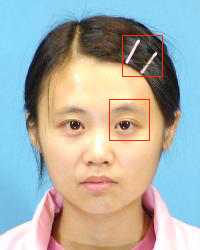
\includegraphics[width=1\linewidth]{img/example_photo.png}
(a) Photo
\end{minipage}
\begin{minipage}[t]{0.24\linewidth}
\centering
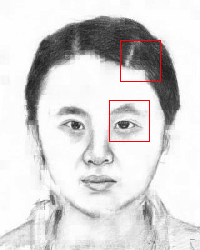
\includegraphics[width=1\linewidth]{img/example_mrf.png}
(b) MRF\cite{wang2009face}
\end{minipage}
\begin{minipage}[t]{0.24\linewidth}
\centering
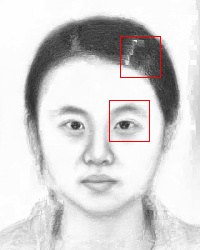
\includegraphics[width=1\linewidth]{img/example_wmrf.png}
(c) WMRF\cite{zhou2012markov}
\end{minipage}
\begin{minipage}[t]{0.24\linewidth}
\centering
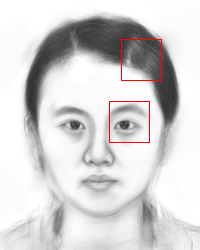
\includegraphics[width=1\linewidth]{img/example_ssd.png}
(d) SSD\cite{song2014real}
\end{minipage}
\begin{minipage}[t]{0.24\linewidth}
\centering
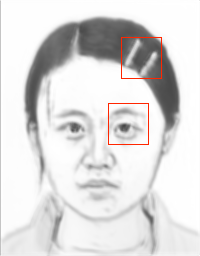
\includegraphics[width=1\linewidth]{img/example_fcnn.png}
(e) FCNN\cite{zhang2015end}
\end{minipage}
\begin{minipage}[t]{0.23\linewidth}
\centering
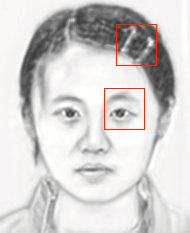
\includegraphics[width=1\linewidth]{img/example_bfcn.png}
(f) BFCN \cite{zhang2017content}
\end{minipage}
\begin{minipage}[t]{0.24\linewidth}
\centering
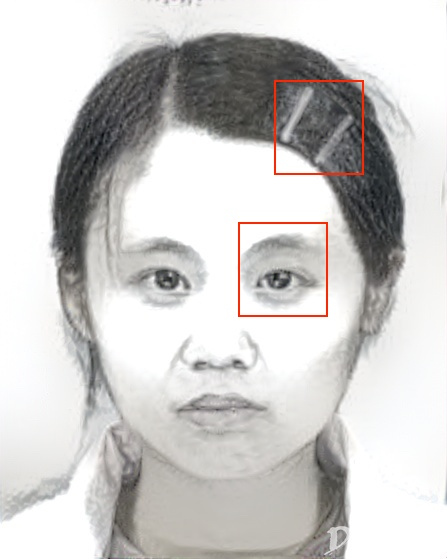
\includegraphics[width=1\linewidth]{img/example_deepart.jpg}
(h) \cite{gatys2015neural}$^*$
\end{minipage}
\begin{minipage}[t]{0.24\linewidth}
\centering
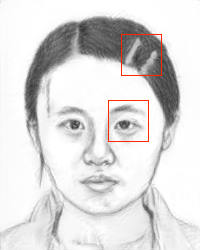
\includegraphics[width=1\linewidth]{img/example_ours.png}
(g) Ours
\end{minipage}
\begin{minipage}[t]{1\linewidth}
\centering
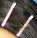
\includegraphics[width=0.11\linewidth]{img/hairpin_photo_patch.png}
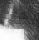
\includegraphics[width=0.11\linewidth]{img/hairpin_mrf_patch.png}
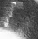
\includegraphics[width=0.11\linewidth]{img/hairpin_wmrf_patch.png}
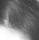
\includegraphics[width=0.11\linewidth]{img/hairpin_ssd_patch.png}
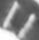
\includegraphics[width=0.11\linewidth]{img/hairpin_fcnn_patch.png}
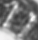
\includegraphics[width=0.11\linewidth]{img/hairpin_bfcn_patch.png}
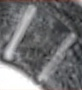
\includegraphics[width=0.11\linewidth]{img/hairpin_deepart_patch.jpg}
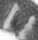
\includegraphics[width=0.11\linewidth]{img/hairpin_ours_patch.png}
\end{minipage}
\begin{minipage}[t]{1\linewidth}
\centering
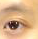
\includegraphics[width=0.11\linewidth]{img/eye_photo.png}
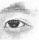
\includegraphics[width=0.11\linewidth]{img/eye_mrf.png}
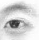
\includegraphics[width=0.11\linewidth]{img/eye_wmrf.png}
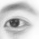
\includegraphics[width=0.11\linewidth]{img/eye_ssd.png}
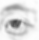
\includegraphics[width=0.11\linewidth]{img/eye_fcnn.png}
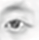
\includegraphics[width=0.11\linewidth]{img/eye_bfcn.png}
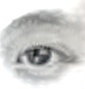
\includegraphics[width=0.11\linewidth]{img/eye_deepart.jpg}
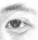
\includegraphics[width=0.11\linewidth]{img/eye_ours.png}
\end{minipage}
\caption[Caption for LOF]{Face sketches generated by existing methods and the proposed method. Our method can not only preserve both hair and facial content, but also maintain sharp textures. \setcounter{footnote}{0} (h)$^*$ is obtained from deep art website\footnotemark~by using the photo as content and a sketch from training set as style.}
\label{fig:example_comp}
\end{figure}
\footnotetext{\url{https://deepart.io/}} 

Unfortunately, there exists no easy solution to face sketch synthesis due to the big stylistic gap between photos and sketches. In the past two decades, a number of exemplar based methods~\cite{wang2009face,song2014real, zhang2010lighting,zhou2012markov} were proposed. In these methods, an input photo is divided into patches and candidate sketches for each photo patch are selected from a training set. The main drawback of such kind of methods is that if the test image can't find a similar patch in the training set, they may lose some contents in the final result. For example, the sketches in the first row of Fig.\ref{fig:example_comp} fail to keep the hairpins. Besides, some methods \cite{song2014real,zhou2012markov} clear away the textures when they try to eliminate the inconsistency between neighboring patches. Another potential risk is that the result may not look like the original photo, \eg left eye in Fig.~\ref{fig:example_comp} (b). Recently, approaches \cite{zhang2017content,zhang2015end} based on convolutional neural network (CNN) were developed to solve these problems. Since these models directly generates sketches from photo, they can maintain the structures and contents of the photos. However, the loss function of them are usually mean square error (MSE) or variation of it, which is responsible for the blur effect, \eg Fig.~\ref{fig:example_comp} (e) and (f). The reason is that MSE prefers values close to mean, and is not suitable for texture representations. The popular neural style transfer provides a better solution for texture synthesis. But there are two obstacles towards directly applying such kind of method. First, it is easily influenced by illumination of the photo, see the face of Fig. \ref{fig:example_comp} (h). Second, it needs a style image to give the global statistics of textures. If the given style doesn't coincide with target sketch, which we don't have, some side effects will occur, \eg the nose in Fig. \ref{fig:example_comp} (h). Extensive experiment and discussion is given in Section~\ref{key}. 

For an artist, the procedure of sketching a face usually starts with outlining the shape of the key facial features like the nose, eyes and mouth. Textures and shadings are then added to regions such as hair lips, and bridge of the nose to give sketches a specific style. Inspired by this and neural style transfer \cite{gatys2015texture}, we propose a new framework for face sketch synthesis that can overcome the aforementioned limitations. In our method, the outline of a face is delineated by a feed-forward neural network, and textures and shadings are then added by a style transfer approach. Specifically, we design a new architecture of Fully Convolutional Neural Network (FCNN) which contains inception layers \cite{szegedy2015going} and convolution layers with batch normalization~\cite{Sergey2015batch} to outline the face (Section \ref{key}). For the texture part, we first divide the feature maps of the target sketch in each layer into a fixed size grid and combine features from different layers but at the same grid location into a pyramid feature column (Section \ref{key}). These pyramid feature columns can be generated by local sketch patches from the training set. A target style is then computed by assembling these pyramid columns. Since we only want the statistics characteristics of these local sketch patches similar to the target sketch, it is not difficult to find them (Section \ref{key}). Our approach is superior to the current state-of-the-art methods in that 
\begin{itemize}
\item It is capable of generating more stylistic sketches without introducing over smoothing artifacts 
\item It can well preserve the content of the test photo.
\end{itemize}

%------------------------------------------------------------------------
\section{Related Work}

\subsection{Face Sketch Synthesis}

Based on the taxonomy of previous studies~\cite{song2014real,zhou2012markov}, face sketch synthesis methods can be roughly categorized into profile sketch synthesis methods~\cite{berger2013style,chen2001example,xu2008hierarchical} and shading sketch synthesis methods~\cite{liu2005nonlinear,song2014real,tang2003face,wang2009face,zhang2015end,zhang2010lighting,zhou2012markov}. Compared with profile sketches, shading sketches are more expressive and thus more preferable in practice. Based on the assumption that there exists a linear transformation between a face photo and a face sketch, the method in~\cite{tang2003face} computes a global eigen-transformation for synthesizing face sketches from face photos. This assumption, however, does not always hold since the modality of face photos and that of face sketches are quite different. Fortunately, Liu et al.~\cite{liu2005nonlinear} found that the linear transformation holds better locally and therefore they proposed a patch based method to perform sketch synthesis. A MRF based method~\cite{wang2009face} was proposed to preserve large scale structures across sketch patches. Variants of the MRF based methods were introduced in~\cite{zhang2010lighting,zhou2012markov} to improve the robustness to lighting and pose, and to render the ability of generating new sketch patches. In addition to these MRF based methods, approaches based on guided image filtering~\cite{song2014real} and feed-forward convolutional neural network~\cite{zhang2015end} are also found to be effective in transferring photos into sketches.

\subsection{Style Transfer with Convolution Neural Network}

The class of Convolutional Neural Networks (CNN) is perhaps the most powerful tool in image processing. It usually contains layers of filters each of which extracts a certain feature from the input or from the output of the previous layer. The VGG-Network~\cite{simonyan2014very}, one popular instance of such networks, rivals human performance in image classification tasks. This demonstrates the ability of CNN in feature extraction. In~\cite{gatys2015texture,gatys2015neural}, Gatys et al. studied the use of CNN in style representation where a target style is computed based on features extracted from an image using the VGG-Network and an output image is generated by minimizing the difference between its style and the target style. Likewise, a perceptual loss function measuring the difference in style between a targeting image and images generated from a CNN was proposed in~\cite{feifei2016} and it was then exploited in the CNN training stage. Our style transfer mechanism is inspired by but different from these works~\cite{gatys2015texture,gatys2015neural,feifei2016} in that our target style is extracted from many images rather than from a single style image. Note that there usually does not exist a single style image in the training set that matches all properties of the test image. Hence, we propose computing the target style based on multiple images. The difficulty of generating a target style from multiple images lies in the non-linearity of the neural network.

%------------------------------------------------------------------------
\section{Final copy}

You must include your signed IEEE copyright release form when you submit
your finished paper. We MUST have this form before your paper can be
published in the proceedings.

Please direct any questions to the production editor in charge of these
proceedings at the IEEE Computer Society Press: Phone (714) 821-8380, or
Fax (714) 761-1784.

{\small
\bibliographystyle{ieee}
\bibliography{egbib}
}

\end{document}
